\documentclass[15pt]{ctexart}
\usepackage{float}
\usepackage{listings}
\usepackage{graphicx}
\usepackage{appendix}
\usepackage[colorlinks]{hyperref}
\usepackage{amsmath}
\usepackage{indentfirst}
\usepackage{enumerate}
\usepackage{fancyhdr}
\usepackage{textcomp}
\usepackage{appendix} 
\usepackage{multirow}
\usepackage{geometry}
\geometry{verbose,letterpaper}
\usepackage{media9}
\pagestyle{fancy}
\lhead{应用层——C/S与P2P通信}
\rhead{\thepage}
\cfoot{}
\lstset{frameshape={RYRYNYYYY}{yny}{yny}{RYRYNYYYY}, backgroundcolor=\color[RGB]{245,245,244}}

\begin{document}
    \begin{titlepage}
    \centering
    
\includegraphics[width=1\textwidth]{imgs/SYSULogo.png}\par\vspace{1cm}
    \vspace{1cm}
    {\scshape\huge 应用层通信 \\ 项目报告 \\ \centering \scshape \Huge C/S与P2P通信 \par}
    \vspace{1.5cm}
    {\Large\bfseries \flushleft 学院:数据科学与计算机学院 \\ 专业:计算机科学与技术 \\ 年级:2016级 \\组长(学号):王锡淮(16337236)\\组员(学号):杨陈泽(16337271)\\
    组员(学号):肖遥(16337258)\par}
    % \vspace{2cm}

% Bottom of the page
    % {\large \today\par}
\end{titlepage}
    \tableofcontents
    \newpage
    \section{项目介绍} % (fold)
    \label{sec:项目介绍}
    \par 这是一个应用层的通信应用项目,包括一个服务器-客户端模型和P2P模型,两者的功能都是传输文件,项目主页是\url{https://github.com/Leo-xh/C-S-and-P2P-demo}。其中,服务器-客户端模型使用的是单服务器多客户端模型,并且单一客户端可以同时请求多个文件,服务器和客户端都使用多线程模型。P2P模型参考的是bittorrent协议,完成了bittorrent协议的一个实现(命名为Compact Bittorrent Protocol/1.0),并且实现了原来的biitorrent协议中的几个扩展协议。
    % section 项目介绍 (end)
    \section{C/S通信} % (fold)
    \label{sec:c_s通信}
    	\par 本项目中实现的C/S通信模型使用python实现,主要利用的是socket,threading,struct,os等常用库,其中服务器使用多线程,能够支持多个客户端同时请求文件;客户端也使用多线程,能够同时请求多个文件。
    	\par 提供的服务如下:
    	\begin{enumerate}[1.]
    		\item 原始数据传输。
    		\item 加密数据传输。
    		\item 查看服务器的文件目录。
    	\end{enumerate}
	    \subsection{协议设计} % (fold)
	    \label{sub:协议设计}
    	\par 这是一个二进制模糊边界和固定边界的协议,即传输的数据以二进制编码,在请求报文中能狗确定报文长度,在应答报文中无法明确知道协议报文的长度,需要通过报文中的长度字段知道。
	    	\par 客户端的请求报文设计如表\ref{tab:client}所示。
	    	\begin{table}[H]
	    		\centering
		    	\begin{tabular}{|c|c|c|c|}
		    		\hline
		    		类型 &服务 &版本 &序号 \\
		    		\hline
		    		\multicolumn{4}{|c|}{\multirow{6}*{文件名}
		    		}
		    		\\
		    		\multicolumn{4}{|c|}{~}\\
		    		\multicolumn{4}{|c|}{~}\\
		    		\multicolumn{4}{|c|}{~}\\
		    		\multicolumn{4}{|c|}{~}\\
		    		\multicolumn{4}{|c|}{~}\\
		    		\multicolumn{4}{|c|}{~}\\
		    		\multicolumn{4}{|c|}{~}\\
		    		\hline
		    	\end{tabular}
		    	\caption{客户端请求报文}
		    	\label{tab:client}
	    	\end{table}
	    	\par 参数解释如下:类型指的是协议号,服务是服务号(3种不同的服务),版本是协议版本号,序号是请求序号,大小都是2字节,文件名指的是请求的文件名,长度上限为200字节。
	    	\par 服务器响应报文设计如表\ref{tab:server}:
	    	\begin{table}[H]
	    		\centering
		    	\begin{tabular}{|c|c|c|c|c|c|}
		    		\hline
		    		类型 &服务 &版本 &序号 &长度 &错误码\\
		    		\hline
		    		\multicolumn{6}{|c|}{\multirow{6}*{数据}}
		    		\\
		    		\multicolumn{6}{|c|}{~}\\
		    		\multicolumn{6}{|c|}{~}\\
		    		\multicolumn{6}{|c|}{~}\\
		    		\multicolumn{6}{|c|}{~}\\
		    		\multicolumn{6}{|c|}{~}\\
		    		\multicolumn{6}{|c|}{~}\\
		    		\multicolumn{6}{|c|}{~}\\
		    		\hline
		    	\end{tabular}
		    	\caption{服务器应答报文}
		    	\label{tab:server}
	    	\end{table}
	    	\par 类型、服务、版本、序号字段和请求报文中一样,长度字段指的是数据字段的长度,大小为2字节,数据字段是发送往客户端的数据。
	    	\par 对于上面提到的三种服务,对应的服务号分别是0,1,2。
	    	\par 服务器和客户端的控制流程如图\ref{fig:server}和\ref{fig:client}所示。
	    	\begin{figure}[H]
	    		\begin{minipage}{0.5\linewidth}
		    		\flushleft
		    		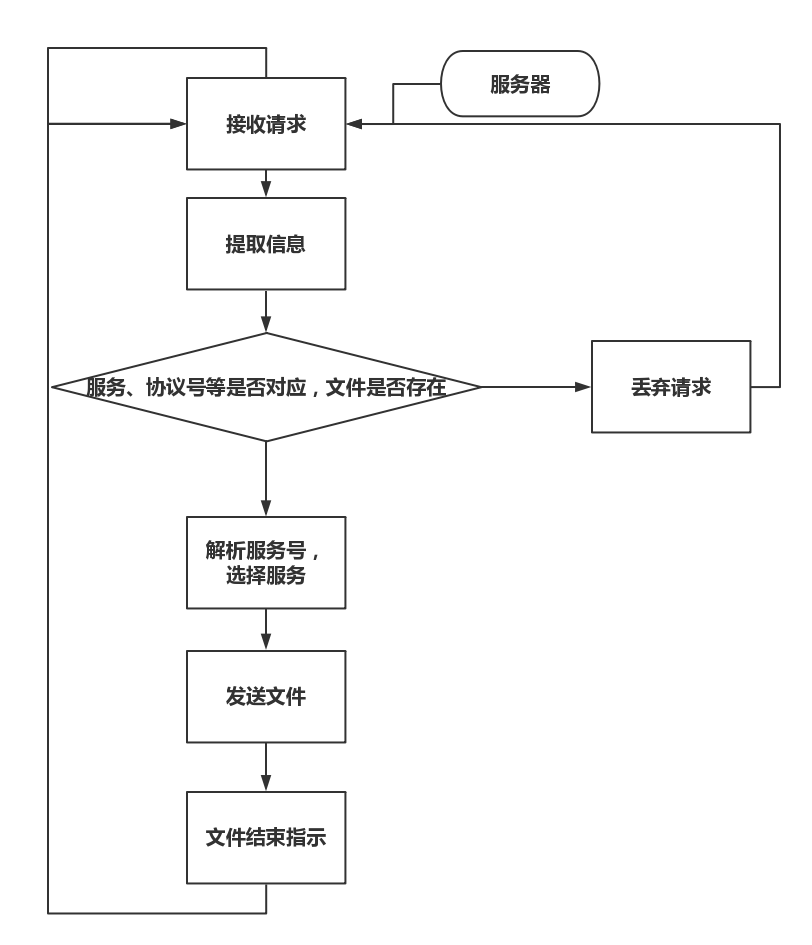
\includegraphics[width=1.1\linewidth]{imgs/server.png}
		    		\caption{服务器流程图}
		    		\label{fig:server}
	    		\end{minipage}
	    		\begin{minipage}{0.45\linewidth}
		    		\flushright
		    		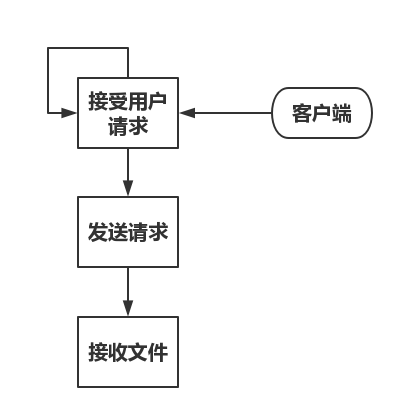
\includegraphics[width=1\linewidth]{imgs/client.png}
		    		\caption{客户端流程图}
		    		\label{fig:client}
	    		\end{minipage}
	    	\end{figure}
	    	\par 在实现这个通信模型时遇到的问题主要是TCP协议的分包和粘包问题,TCP中只有数据流这样的概念,而没有数据包一类的概念,每次收到的不一定会是一个完整的数据包,所以需要通过某种方法明确当前处理的数据包的大小,然后解析这个大小的数据包。
	    % subsection 协议设计 (end)
    	
    	
    % section c_s通信 (end)
	
	\section{P2P通信} % (fold)
	\label{sec:p2p通信}
		\subsection{协议设计} % (fold)
	    \label{sub:协议设计}
	    % subsection 协议设计 (end)


	% section p2p通信 (end)

	\section{安装和部署} % (fold)
	\label{sec:安装和部署}
	
	% section 安装和部署 (end)
    
    \section{结果} % (fold)
    \label{sec:结果}
    	\subsection{结果展示} % (fold)
    	\label{sub:结果展示}
    	\par """"插入结果展示""""
    	\\
    	\\
    	\\
    	\\
    	\\
    	\\
    	\\
    	\\
    	\\
    	\\
    	\\
    	% subsection 结果展示 (end)
    	\subsection{对比} % (fold)
    	\label{sub:对比}
    	
    	% subsection 对比 (end)

    % section 结果 (end)
    \section{总结} % (fold)
    \label{sec:总结}
    
    % section 总结 (end)
   
   \section{项目管理记录} % (fold)
   \label{sec:项目管理记录}
   
   % section 项目管理记录 (end)

    \newpage
    \appendixpage
    \begin{appendices}
        \section{参考文献} % (fold)
            \begin{enumerate}
            	\item 	Jonas Fonseca,et al,\url{http://jonas.nitro.dk/bittorrent/bittorrent-rfc.html#anchor17},Bittorrent协议详细解读。
            \end{enumerate}
        % section  (end)
    \end{appendices}

\end{document}